\documentclass[10pt,a4paper]{article}
\usepackage[margin=2.2cm]{geometry}
\usepackage{fontspec}
\usepackage{kotex}
\setmainfont{Apple SD Gothic Neo}
\setsansfont{Apple SD Gothic Neo}
\usepackage{amsmath,amssymb}
\usepackage{graphicx}
\usepackage{caption}
\usepackage[dvipsnames]{xcolor}
\usepackage[colorlinks=true,linkcolor=MidnightBlue,citecolor=MidnightBlue,
            urlcolor=MidnightBlue]{hyperref}
\usepackage{titlesec}
\titleformat{\section}{\large\bfseries}{\thesection}{0.6em}{}
\captionsetup{font=small,labelfont=bf}
\setlength{\parskip}{0.35em}
\setlength{\parindent}{0pt}
\usepackage{mdframed}
\newmdenv[linewidth=0.4pt,linecolor=gray!60,backgroundcolor=gray!5,
          innertopmargin=6pt,innerbottommargin=6pt,skipabove=8pt,skipbelow=8pt]{claimbox}
\newcommand{\claim}[2]{\begin{claimbox}\textbf{주장.} #1\par\smallskip
  \textcolor{gray!70}{\textbf{반증 조건.} #2}\end{claimbox}}

\title{\bfseries 가르는 것을 모른다, 가 최종 답이다\\[2pt]
\large $808$ 문패 종결 --- $n=12$ 에서도 단일 지표는 없다}
\author{월드모델 실험실 · 노트 $840$}
\date{2026-08-08}
\begin{document}\maketitle

\section{한 줄}

$808$ 이 문패로 걸어 둔 재개 조건($n=12$)이 채워져 원문 규칙 그대로 다시
쟀다: 도메인별 절대값 승부(유보백분위 $-$ 기후값 자릿수 오차 차) 대 후보
둘. \textbf{드리프트 $r = +0.259$ · 왜도 $r = +0.406$ --- 둘 다 문턱
$0.75$ 미달 $\to$ (없) · 문패 종결.} 예측($65\%$) 적중. ``무엇이 절대값
승부를 가르는지 모른다''가 $n=11$ 의 잠정이 아니라 \textbf{최종 기록}이
됐고, 능력 카드의 절대값 문구(드리프트 보정 $+$ 자 병기)는 그대로가 정직하다.

\begin{figure}[t]\centering
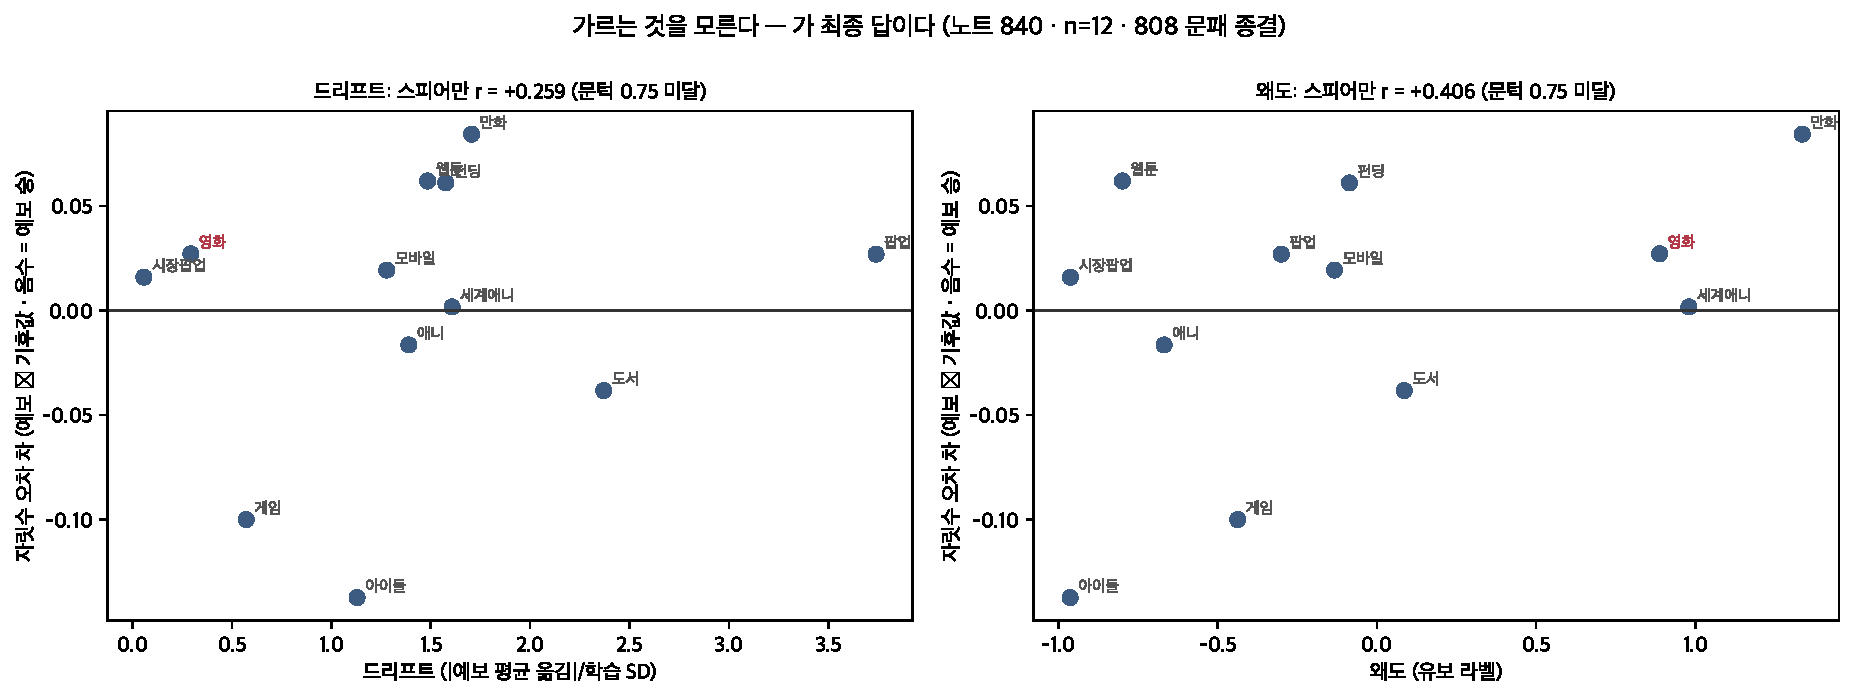
\includegraphics[width=0.97\textwidth]{figs/unknown.pdf}
\caption{두 후보 대 절대값 승부 --- $n=12$. 붉은 라벨이 새 데이터점(영화).}
\end{figure}

\claim{\textbf{영화 데이터점의 정직}: 자릿수차 $+0.0271$ --- 기후값이 소폭
이긴다(내 부 예측 `예보 승 $60\%$' 틀림 --- $21$일 고정 창 라벨은 연도
기후값이 강한 구조다). 드리프트 $0.292$ 는 판 최소급(적중 --- 학습 $2$년 ·
동일 수집원). T$6$ 은 이것으로 완전 종결(사슬 $791{\sim}809$ $+$ 문패 $808$).}
{남은 문패는 둘: $819$(조건부 치환) · $822$(재상관) --- $841{\sim}$. GitHub
흐름 $3$회째 완주(이슈 \#$6 \to$ PR \#$7$). 판 $\rho$ $0.4710$ 그대로.}

\end{document}
